\chapter{Interfaces with \dword{lbnf}}
\label{vl:tc-lbnf}

\section{Organization of Interfaces}
\label{sec:inter-org-interf}
In order to manage interfaces within the detector and between the
detector and facilities, an overall integration mechanism has been
developed which consist of integration nodes. Each node is integrated
and managed by a specific group. The interfaces between the nodes are
managed by the \dword{tc} engineering team.

Figure~\ref{fig:integration_nodes} shows the interfaces between the
detector and facilities.
\begin{dunefigure}[Integration Nodes.]{fig:integration_nodes}
  {Overall Integration Nodes and Interfaces.}
  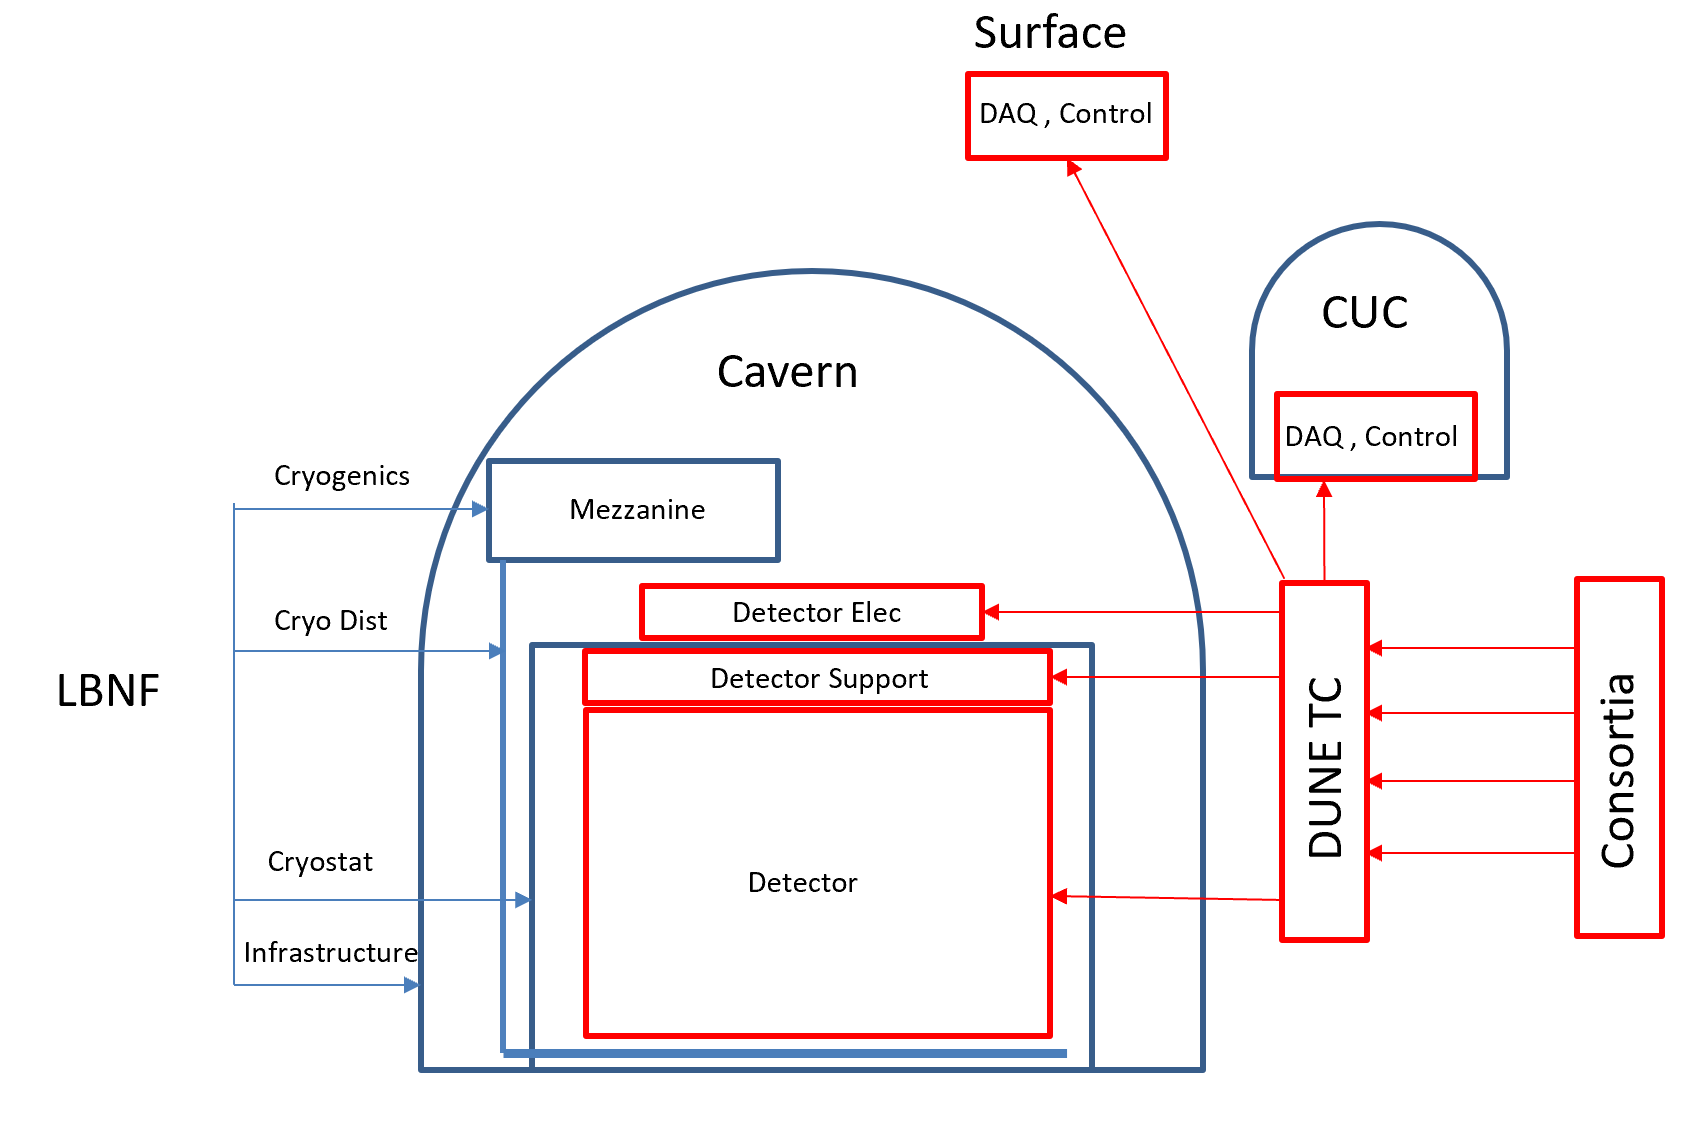
\includegraphics[width=0.7\textwidth]{Integration_nodes.png}
\end{dunefigure}
Within the cavern items provided by \dword{lbnf} are
represented on the left and the items provided by \dword{dune} are represented
on the right. In addition, \dword{tc} engineering team is also
responsible for the integration of the DAQ room in the Central Utility
Cavern and surface control and network rooms. Interfaces with \dword{lbnf} are
managed at the boundaries of each integration node. As an example,
interface between \dword{lbnf} and \dword{dune} for the underground DAQ and control
rooms are power, cooling water, data fibers, cable penetrations at the
room boundaries. The implementation of power, cooling water, data and
signal cables, and rack integration are the responsibilities of \dword{dune}.


The integration nodes consists of the following:
\begin{itemize}
\item {\bf Detector:} All TPC elements within LAr All Consortia involved in
  this integration task which is mostly mechanical. Consortia
  engineering work directly with \dword{tc} engineering team.
  Interface with DSS though hangers. Examples of interfaces within
  this node are field cage connections to both CPAs and APAs, CE and
  PD cable routing within cryostat and location of calibration and
  cryogenic instrumentation.
\item {\bf Detector Support System (DSS):} All detector support elements,
  cable trays and feedthroughs.
\item {\bf Detector Electronics:} All racks, cooling, power, cable
  trays and cable distribution on top of cryostat, rack protection
  (smoke detectors, hardware power trip), rack build, determination on
  how to best load electrical hardware into the racks, interface to
  building safety systems
\item {\bf DAQ and Electronics:} Electronics on top of cryostat and
  the CUC DAQ room and surface rooms, fiber Optic distribution from
  the surface to the CUC DAQ room, fiber Optic distribution from the
  detectors to the CUC DAQ Room, layout and cooling of the CUC DAQ
  room
\end{itemize}

\section{Interfaces with \dword{lbnf}}
\label{sec:inter-lbnf-interf}
The following figures and explanations are intended to show the
integration of the detector modules within the cavern. The interfaces
boundaries are not pointed out specifically in each figure, but they
follow the scheme as represented in
Figure~\ref{fig:integration_nodes}.

Figure~\ref{fig:detector_cavern} shows one detector module within the
cavern. In this figure the cryogenics equipment and racks on top of
the detector are visible. The LAr recirculation pumps can also be seen
o the lower lever.
\begin{dunefigure}[Overall view of the detector in cavern.]{fig:detector_cavern}
  {Overall view of the a detector module within the cavern.}
  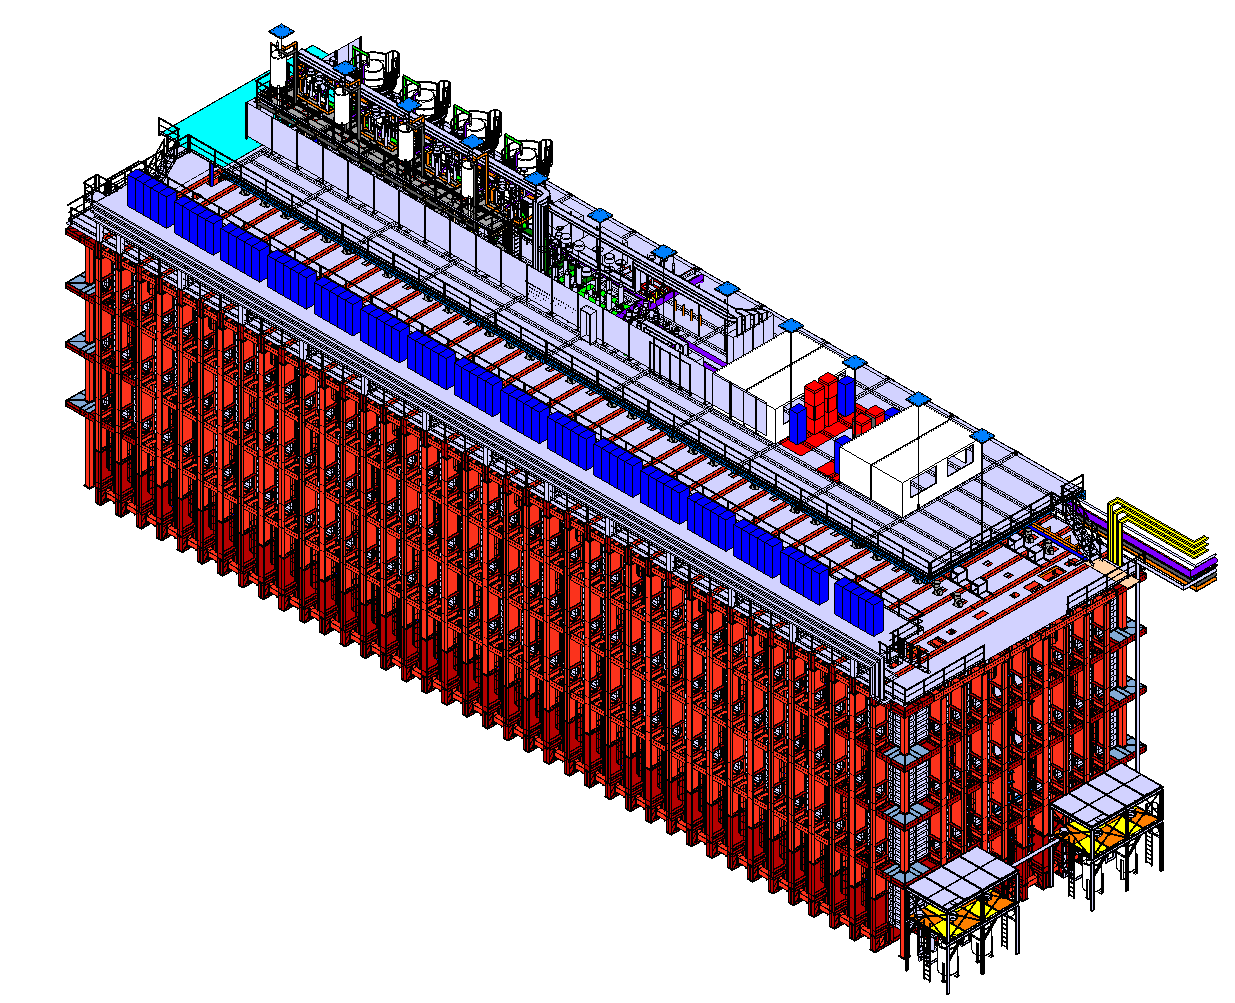
\includegraphics[width=0.8\textwidth]{LBNF-Cryostat-NW_Iso_c.png}
\end{dunefigure}

Figure~\ref{fig:detector_ew_elevation} shows the elevation view of the
detector within the cavern from east to west. The services from the
CUC enter the cavern through a passage that is visible on the left.
\begin{dunefigure}[East-west elevation view of Detector]{fig:detector_ew_elevation}
  {East-west elevation view of one detector module within the cavern.}
  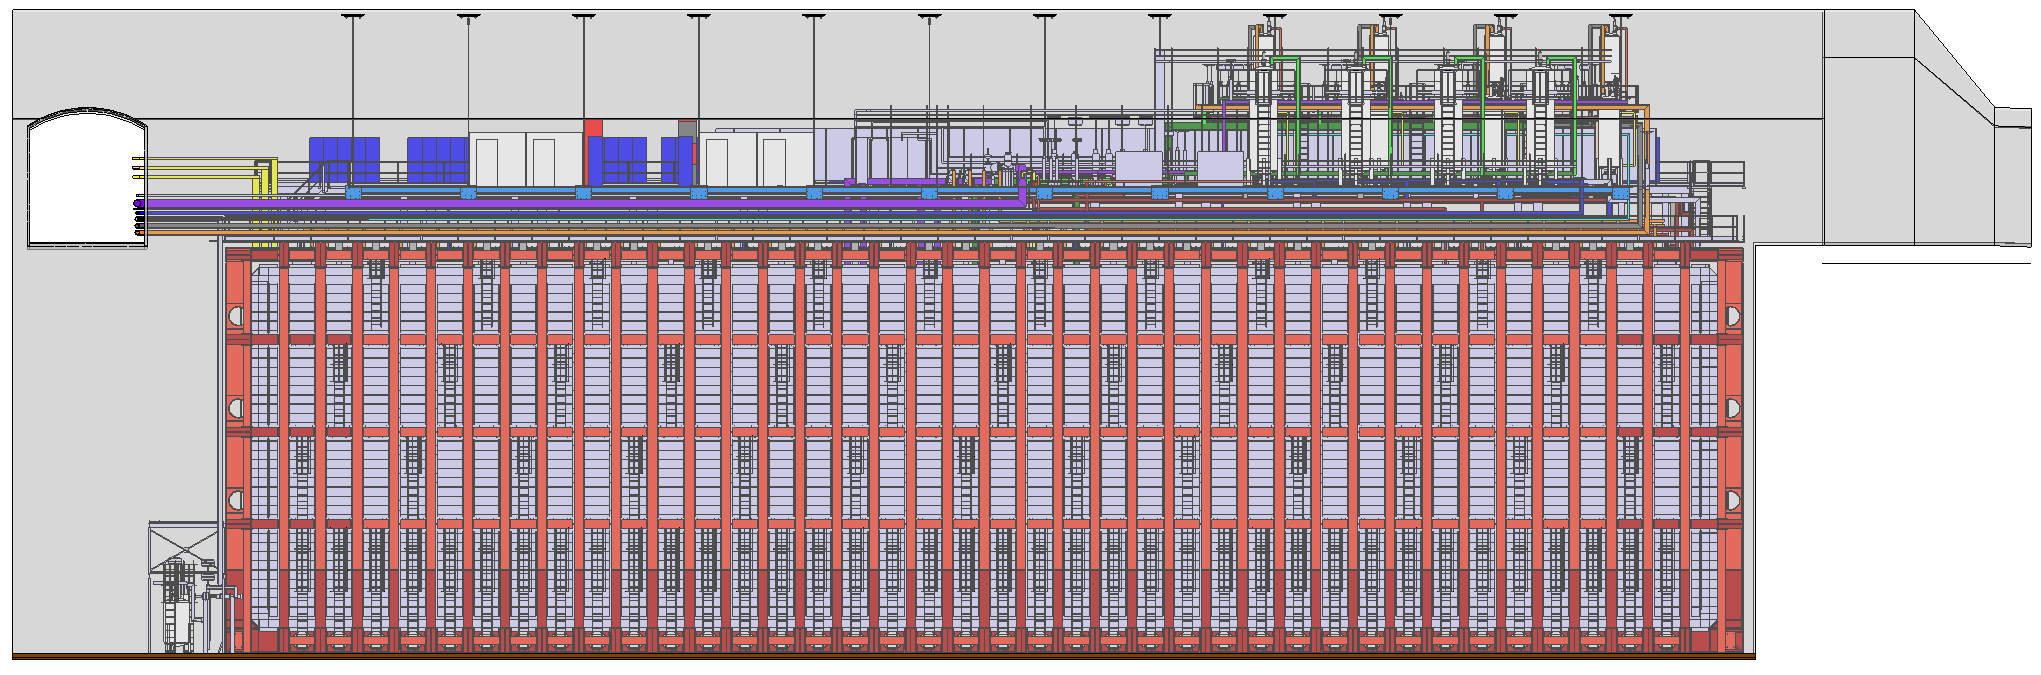
\includegraphics[width=0.9\textwidth]{LBNF-Cryostat-South_Elevation_in_Cavern_c.png}
\end{dunefigure}

Figure~\ref{fig:detector_ns_elevation} shows the elevation view of the
detector within the cavern from north to south. The services entering
from the CUC are visible on the right.
\begin{dunefigure}[North-south elevation view of detector]{fig:detector_ns_elevation}
  {North-south elevation view of one detector within the cavern.}
  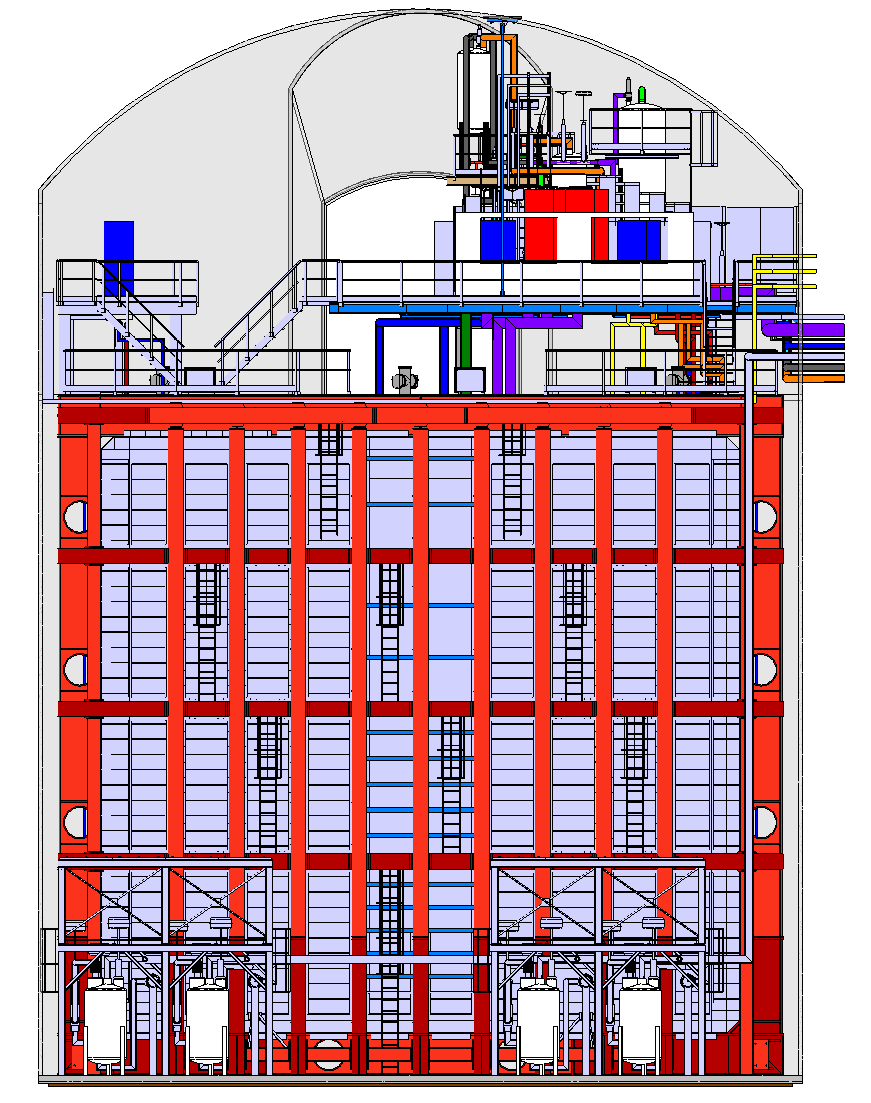
\includegraphics[width=0.7\textwidth]{LBNF-Cryostat-West_Elevation_in_Cavern_c.png}
\end{dunefigure}

Figure~\ref{fig:detector_mezzanines} shows the elevation view of the
top of cryostat showing mezzanines, cryogenic equipment and electronic
racks.
\begin{dunefigure}[Elevation view of top of cryostat showing mezzanines, cryogenic
    equipment and electronic racks.]{fig:detector_mezzanines}
  {Elevation view of top of cryostat showing mezzanines, cryogenic
    equipment and electronic racks.}
  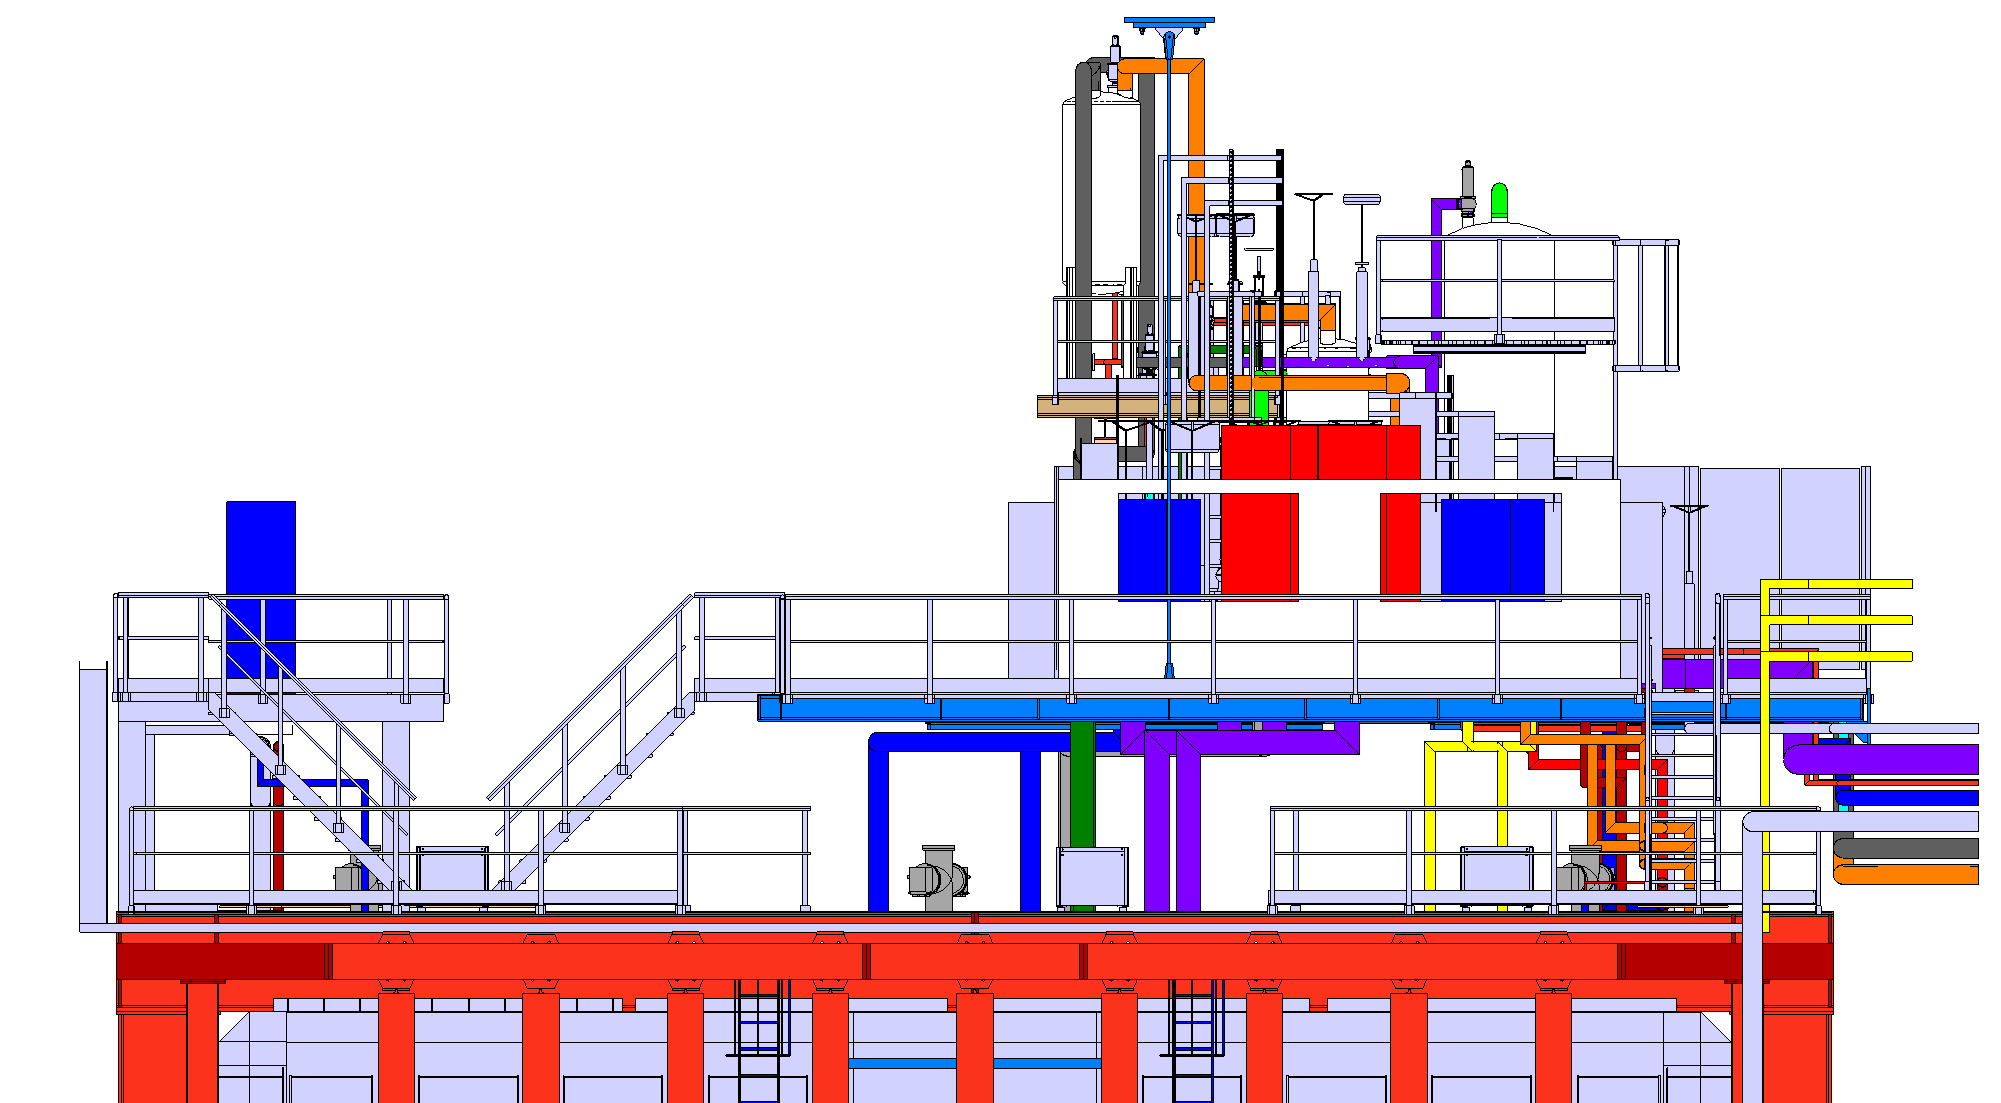
\includegraphics[width=0.85\textwidth]{LBNF-Cryostat-West_Elevation-Cryo_c.png}
\end{dunefigure}
The cryogenics are installed on a mezzanine which is supported from
the cavern roof and cavern wall. Cryogenic distribution lines are
routed under the mezzanine. There are also local control rooms for the
cryogenic equipment on the mezzanine.

Detector electronics are installed in short racks close to
feedthroughs and in taller racks, which are installed on a separate
electronics gallery shown on the left. This will allow for good access
and maintenance and reduce complexity on top of the detector.
